\documentclass[a4paper]{paper}
\usepackage[utf8]{inputenc}
\usepackage{xcolor}
\usepackage{graphicx} 

\begin{document}
\title{A look at the health of the Go ecosystem}
\author{Ingvar Mattsson}

\maketitle

\section{Background}

The root inspiration for this investigation and report was trying to
use Athens, with a validating web-hook, for a company concerned with
what is brought in from external sources.

In the initial setup, there were three intentional (and one
non-intentional) way a package could fail validation. It could have
file(s) that triggered a vulnerability scanner, it could fail to
build, it could have failing unit tests. Or, unintended, either ``go
mod download'' or ``go list -json'' could fail.

It soon became evident that ``has failing unit tests'' was not a
feasible\footnote{Part of this is that over time, multiple ``go vet''
  errors ave been promoted test errors} criterion. It eventually
became evident that ``has failing build targets'' was also not
feasible.

This raised a question in the author's mind. What is the current state
of health of the Go eco-system?

\section{Methodology}

In order to investigate what the current state of health of the Go
eco-system, you need to compile a lot of Go packages. You also need to
do some statistics on them.

In order to more easily get multiple modules, at various versions,
compiled through an instrumented build environment, the author built
an environment consisting of a validator (custom Go code), Athens
(pre-existing Docker container), and an instrumented build environment
(Python, in a Docker container).

\begin{figure}[ht]
  \label{fig:architecture}
  \caption{Rough system architecture, depicting JSON requests, module requests and execution with different arrows}
  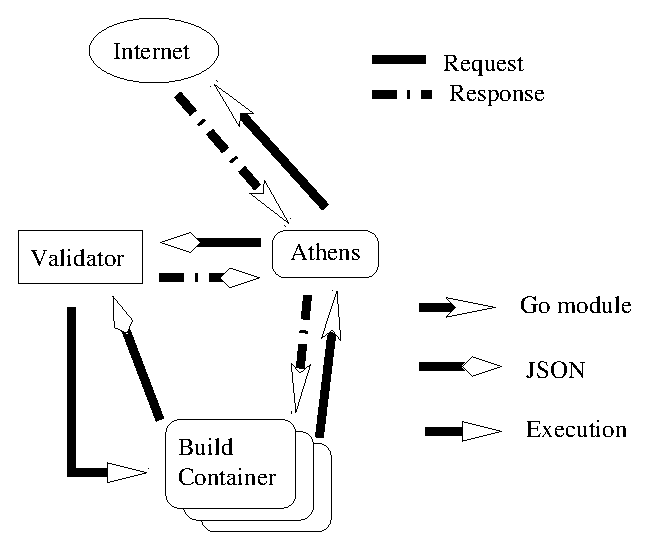
\includegraphics{architecture.eps}
\end{figure}


The validator considers all module/version tuples as valid. If the
specific module/version tuple has not been seen before, a build of
that is started. The validator limits builds to at most five
concurrent ones, this is to preserve some responsitivity on the test
machine. It is possible to increase the build parallelism by having
more ``build workers''. The number of build workers is set at build
time.

The custom build environment then reports back some general statistics
(did ``go mod download'' work, did all builds succeed, did all tests
succeed, how many build/test targets, and (on failure) what build/test
targets failed). The build environment is set up to use the Athens
instance as its GOPROXY, making it much easier to get a wide spectrum
of code scanned.

The validator periodically writes its current data set to disk. There
is also a web endpoint that triggers a save. The validator will only
create a new safe file if there's been any changes since the last
save.

To seed the scan, a few packages were manually started within the
build container, using the same environment as that set up by the
validator. For more details, see the section on seed packages.

The source code for the tabulator, the validation webhook framework
and the build instrumentation can be found at
https://github.com/vatine/gochecker/.

\section{The numbers}

Here are some numbers distilled from the investigation. For the
breakdown on failing build/test cases, the mean has only been done for
module/versions with at least one failure. The number of packages with
download problems is over-reported, as it includes: packages with a
name that differs from the requested in their go.mod, packages with a
version number that doesn't parse, and packages that simply do not
exist at this point in time.

\begin{table}[ht]
\caption{Build target statistics}
\label{table:build}
\begin{tabular}{|l|r|}
 \hline
  Packages processed & 5086 \\
  Packages failed to download & 117 \\
  No build failures & 4552 (89.500590\%) \\
  No vet failures & 2994 (58.867479\%) \\
  No test targets & 762 (14.982304\%) \\
 \hline
  Mean build targets (all modules)& 38.503146 \\
  stddev & 126.801294 \\
  Median build targets & 4 \\
  75th percentile \# of build targets & 24 \\
  90th percentile \# of build targets & 133 \\
  95th percentile \# of build targets & 185 \\
  99th percentile \# of build targets & 449 \\
  Max \# of build targets & 2200 \\
 \hline
  Mean build targets (at least one buildable)& 39.834622 \\
  stddev & 128.769733 \\
 \hline
  Mean failed build targets (all modules)& 5.367283 \\
  stddev & 46.321543 \\
 \hline
  Mean failed build targets (at least one failed)& 51.119850 \\
  stddev & 134.637700 \\
 \hline
  Mean failed vet targets (all modules)& 6.410932 \\
  stddev & 46.941213 \\
 \hline
  Mean failed vet targets (at least one failed)& 16.964620 \\
  stddev & 75.190439 \\
 \hline
\end{tabular}
\end{table}

\begin{table}[ht]
\caption{Test target statistics}
\label{table:test}
\begin{tabular}{|l|r|}
 \hline
  Packages seen & 5086 \\
  No test failures & 3334 (65.552497\%) \\
  No test failures (with tests) & 2572 (59.481961\%) \\
  No build failures, but test failures & 1319 (25.933936\%) \\
  No tests & 762 (14.982304\%) \\
 \hline
  Mean failed test targets for passed builds (all) & 2.334344 \\
  stddev & 2.345298 \\
 \hline
  Mean failed test targets for passed builds (at least one fail) & 2.334344 \\
  stddev & 2.345298 \\
 \hline
  Mean failed test targets, all packages& 5.455479 \\
  stddev & 14.724862 \\
 \hline
  Mean failed test targets, packages with at least one test failure& 5.455479 \\
  stddev & 14.724862 \\
 \hline
\end{tabular}
\end{table}

\begin{table}[ht]
\caption{Most versions per module that  download}
\label{table:versions}
\begin{tabular}{|l|r|}
\hline
 golang.org/x/tools & 217 \\
 golang.org/x/sys & 132 \\
 golang.org/x/net & 82 \\
 google.golang.org/genproto & 82 \\
 golang.org/x/crypto & 78 \\
 github.com/gobuffalo/genny & 43 \\
 github.com/aws/aws-sdk-go & 39 \\
 k8s.io/apimachinery & 37 \\
 google.golang.org/api & 36 \\
 k8s.io/api & 33 \\
\hline
\end{tabular}
\end{table}
\begin{table}[ht]
\caption{Most versions per module that fail to download}
\label{table:failversions}
\begin{tabular}{|l|r|}
\hline
 github.com/hashicorp/vault/sdk & 3 \\
 knative.dev/test-infra & 3 \\
 knative.dev/pkg & 3 \\
 github.com/operator-framework/operator-sdk & 2 \\
 k8s.io/apiextensions-apiserver & 2 \\
 github.com/openshift/api & 2 \\
 google.golang.org/cloud & 2 \\
 github.com/portworx/sched-ops & 2 \\
 github.com/coreos/prometheus-operator & 2 \\
 k8s.io/client-go & 2 \\
\hline
\end{tabular}
\end{table}


\section{Investigation of (some) build errors}

It is clear that some number of build errors are down to deficiencies
in the build environment. It also does not have OpenGL, ALSA and other
libraries/dependencies installed (this is a major problem for
github.com/hajimehosi/ebiten).

There are some packages that do not work to download with ``go mod
download'', this seems to be down to structural problems with the
repositories, like ``at higher than v1, but not under a v2 (or later)
path prefix. Observing that this is a possible source of ``fewer
transitive dependencies'' as well as ``possibly false failed
download'' numbers, the build environment has been changed to first
try a ``go mod download'', and if that fails, a ``go get'' at the same
version.

Some packages fail because the path declared in their go.mod does not
correspond to the path their dependencies have
declared\footnote{Changing ``full name'' of a Go module is
  problematic, as that effectively changes the ``unique identifier''}.

In some cases, an erroneous version number has snuck in, causing
problems downloading the package\footnote{This seems prevalent for
  packages listing dependencies under k8s.io, for some reason}. One possibility
may be that the go.mod file using local rewrites for
dependencies. These work for the ``root'' package, but do not work
during a transitive build. Another possibility is an automatic attempt to convert a godeps dependency file to a go.mod.

\section{Investigation of (some) test errors}

As a general comment, it is a bit surprising that tagged releases have
test errors at all, indicating that there's improvements to make
around release processes. In some cases, this is because the tooling
has changed what constitutes a ``passing'' test (over time, some ``go
vet'' warnings have become errors when they occur in test files).

We will now look closer at a few packages. I have explicitly excluded
packages that have build failures from closer inspection, as the test
may well be because of one )or more) build failures due to missing
dependencies.

The methodology for choosing packages is (approximately) looking
through the emitted latest data file, in whatever order the JSON
marshalling places things, investigate more closely what the test
warnings are, until it is no longer fun to dig anymore.

\subsection{github.com/AaronO/go-git-http@v0.0.0-20161214145340-1d9485b3a98f}

Go vet warning for two incorrect format strings in the main code.

\subsection{github.com/Azure/azure-sdk-for-go@v35.0.0+incompatible}

Failing to find test fixtures.

Inability to modify the ``pkg/mod'' directory structure (it is
read-only by default).

Unit-test requires running in a got clone, not in a module download

\subsection{github.com/Azure/go-autorest/autorest/adal@v0.1.0}

Multiple errors unmarshalling JSON into structs.

\subsection{github.com/GoogleCloudPlatform/cloudsql-proxy@v0.0.0-20190129172621-c8b1d7a94ddf}

Missing dependencies (specifically, one or more FUSE binaries).

\subsection{github.com/Graylog2/go-gelf@v0.0.0-20170811154226-7ebf4f536d8f}

Not sure about he exact root cause, but it looks like the unit test
expects a very specific build paths.

\subsection{github.com/IBM/keyprotect-go-client@v0.4.0}

String mismatch (the seen string has a few double-quotes that the
expected is missing).

\subsection{github.com/bifurcation/mint@v0.0.0-20180715133206-93c51c6ce115}

A ``go vet'' error in the test code.

\subsection{github.com/bmizerany/perks@v0.0.0-20141205001514-d9a9656a3a4b}

A ``go vet'' error in the test code.

\section{Recommendations based on this research}

\subsection{Renaming}
It is recommended to never rename a Go module. If you want it available
under a new name, consider the new name a ``new module'' and leave
releases up to the point in time where the changed version still
available under the old name. If necessary, archive the repository, so
that no further accidental modifications are possible. Probably after
leaving a link in a README pointing to the new location.

Otherwise, the renaming has suddenly broken previously-fine
packages. If nothing else, the name change is putting a burden on any
user of your library and should ideally be followed up with a pull
request\footnote{The use of github.com as a platform is quite
  prevalent, other version control systems have different names for
  ``this is a unit of change''.} to bring users of the library back to
a building state.

\subsection{Testing}

It is recommended to have pull requests checked against all (or at least all relevant) test targets as part of the review process. Ideally, this should be done by automation, posting status back to the project.

It is strongly recommended to not cut a release if there are any failing unit tests.

\section{Seed packages}

This is the list of every seed package. During the data gathering, a problem with the build environment was noticed and the seed list contains all packages that failed to download due to a name change. Packages that failed ``go mod download'', but worked with ``go get'' have not been listed explicitly, as they would have worked, had that fallback existed from the beginning.

Modules listed as ``due to name change'' have been diagnosed as such because there was a compiler warning signalling that the name in the go.mod file is different from that used to request the module.

Some of the specific module names are considered changed due to Go versions prior to Go 1.11 not really caring about capitalisation, but with go modules this is now considered as different paths.

\begin{table}[ht]
  \caption{Seed modules and versions}
  \label{table:seed}
  \begin{itemize}
  \item github.com/coreos/prometheus-operator v0.39.0
  \item github.com/hajimehoshi/ebiten v1.11.1
  \item github.com/hashicorp/terraform, v0.12.24
  \item github.com/miekg/dns, v1.1.29
  \item github.com/prometheus/alertmanager v0.20.0
  \item go.uber.org/zap v1.15.0

  \item cloud.google.com/go  v0.57.0 (due to changed name)
  \item cloud.google.com/go/logging v1.0.0 (due to changed name)
  \item github.com/caddyserver/caddy v1.0.5 (due to name change)
  \item github.com/containerd/fifo v0.0.0-20200410184934-f15a3290365b (due to name change)
  \item github.com/containerd/ttrpc @ v1.0.1 (due to name change)
  \item github.com/influxdata/influxdb v1.8.0 (due to name change)
  \item github.com/lithammer/dedent v1.1.0 (due to name change)
  \item github.com/openzipkin-contrib/zipkin-go-opentracing v0.4.5 (due to name change)
  \item github.com/sirupsen/logrus v1.6.0 (due to name change)
  \item github.com/sourcegraph/go-diff v0.5.2 (due to changed name)
  \item github.com/unknwon/com v1.0.1 (dure to name change)
  \item github.com/urfave/cli v1.22.4 (due to name change)
  \item go.etcd.io/bbolt v1.3.4 (due to name change)
  \item go.uber.org/atomic v1.6.0 (due to name change)
  \item gopkg.in/resty.v1 v1.12.0 (due to name change)
    
  \end{itemize}
\end{table}


\end{document}
